\documentclass{beamer}
\usepackage[utf8]{inputenc}
\usepackage[spanish]{babel}
\usepackage{amsmath, amssymb, graphicx}
\usepackage{natbib}
\setcitestyle{year,open={(},close={)}}


% Configuración del tema
\usetheme{Madrid}
\usecolortheme{seahorse}

\title{Resolución de Ecuaciones Diferenciales Parciales con Polinomios de Zernike}
\author{Andrés David Cadena Simons}
\institute{Universidad Nacional de Colombia}
\date{\today}

\begin{document}

% Portada
\begin{frame}
    \titlepage
\end{frame}

\begin{frame}{Introducción}
    \begin{itemize}
        \item ¿Por qué resolver EDPs en regiones circulares?
        \item Aplicaciones en óptica, fluidos, electromagnetismo.
        \item Métodos espectrales tradicionales tienen dificultades con condiciones de frontera discontinuas.
        \item Se propone el uso de los polinomios de Zernike, que son ortogonales en el disco unitario y permiten una mejor representación de soluciones en regiones circulares.
    \end{itemize}
    \cite{Datta2022}
\end{frame}

\begin{frame}{Polinomios de Zernike}
    \begin{itemize}
        \item Definición y propiedades.
        \item Expansión en términos de \textbf{parte radial} y \textbf{parte azimutal}.
        \item Comparación con bases ortogonales en el disco unitario.
    \end{itemize}
\end{frame}

\begin{frame}
  Los polinomios de Zernikel han sido usados convenientemente para hablar sobre funciones del tipo ondas ópticas, como ya antes hemos mencionado, estos están definidos sobre el disco unitario $\{(x,y)\in \mathbb{R}^{2}: x^2+y^2\leq 1\}$.\\
  Ellos son solución de la EDP
  \begin{align*}
    \Delta U+\alpha\left( x\frac{\partial }{\partial x}+y\frac{\partial }{\partial y} \right)^2U+\beta\left( x\frac{\partial }{\partial x}+y\frac{\partial }{\partial y} \right)U+\gamma U=0
  \end{align*}
  En coordenadas polares:
  \begin{align*}
    (1+\alpha r^2)\frac{\partial^2 U}{\partial r^2}+\left( \frac{1}{r}+(\alpha+\beta)r \right)\frac{\partial U}{\partial r}+\frac{1}{r^2}\frac{\partial ^2U}{\partial \phi^2}+\gamma U=0
  \end{align*}
\end{frame}

\begin{frame}
  Tomando $\alpha=-1$ y $\beta=-1$, y $\gamma=n(n+2)$ obtenemos la ecuación hipergeométrica
  \begin{align*}
    x(1-x)\frac{d^2y}{dx^2}+(1-2x)\frac{dy}{dx}+\frac{1}{4}\left[ n(n+2)-\frac{m^2}{x} \right]y=0
  \end{align*}
\end{frame}

\begin{frame}
  \begin{enumerate}
  \item Se encuentra en la solución de la ecuación de Schrödinger para ciertos potenciales efectivamente atractivos o confinantes.
  \item Puede modelar la ecuación radial de la función de onda en coordenadas esféricas o parabólicas en problemas de separación de variables.
  \item La presencia del término $\frac{m^2}{x}$ sugiere una relación con las ecuaciones de los armónicos esféricos en coordenadas esféricas.
  \item En algunos casos, se relaciona con la ecuación de Laplace en espacios curvos o con la ecuación de Helmholtz en el contexto de ondas.
  \item En teoría de la difracción y la propagación de ondas electromagnéticas en medios con simetría esférica, aparecen ecuaciones similares.
  \item Está relacionada con los polinomios de Jacobi e hipergeométricos, que aparecen en la expansión de funciones en términos de soluciones de ecuaciones diferenciales especiales.
  \end{enumerate}
\end{frame}

\begin{frame}
  En particular
  \begin{align*}
    U_n^m (r,\phi) = R_n^m (r) (C_1 \cos m\phi + C_2 \sin m\phi), \quad n \in \mathbb{N} \cup \{0\}, \quad n - m \geq 0, \quad n - m \text{ par},
  \end{align*}
  donde
  \begin{align*}
    R_n^m (r) = \sum_{\ell=0}^{\frac{n-m}{2}} (-1)^\ell \frac{(n - \ell)!}{\ell! ( \frac{n-m}{2} - \ell)! ( \frac{n+m}{2} - \ell)!} r^{n-2\ell}.
  \end{align*}
  Son una base que genera un espacio denso en $L^2(B_{1}(0))$.
\end{frame}

\begin{frame}
  En dónde podemos dar la aproximación de una función $f$ como:
\[
f(r,\phi) = \sum_{n=0}^{\infty} \sum_{\substack{0 \leq m \leq n \\ n-m \text{ par}}} (A_{nm} \cos m\phi + B_{nm} \sin m\phi) R_n^m (r)
\]

donde

\[
A_{nm} = \frac{\epsilon_m (n+1)}{\pi} \int_0^1 \int_0^{2\pi} f(r,\phi) \cos m\phi R_n^m (r) r d\phi dr,
\]

\[
B_{nm} = \frac{\epsilon_m (n+1)}{\pi} \int_0^1 \int_0^{2\pi} f(r,\phi) \sin m\phi R_n^m (r) r d\phi dr,
\]

y \(\epsilon_m\) es el factor de Neumann:

\[
\epsilon_m = 
\begin{cases} 
1 & \text{si } m = 0, \\
2 & \text{en otro caso}.
\end{cases}
\]
\end{frame}

\begin{frame}
Una aproximación de \( f \) de orden \((m,n)\) se puede calcular como

\[
f(r,\phi) = \sum_{i=0}^{n} \sum_{\substack{0 \leq j \leq i \\ i-j \text{ par}}} (A_{ij} \cos j\phi + B_{ij} \sin j\phi) R_i^j (r).
\]
\end{frame}

\begin{frame}{Resolución de EDPs de Primer Orden}
    \begin{itemize}
        \item Forma general: $\alpha(x, y) \frac{\partial u}{\partial x} + \beta(x, y) \frac{\partial u}{\partial y} + \gamma(x, y) u = f(x, y)$.
        \item Transformación a coordenadas polares.
        \item Uso de matrices operacionales de integración (IOM) para representar operadores diferenciales.
        \item Expandir \( u(r, \theta) \) en polinomios de Zernike.
        \item Usar la matriz IOM para expresar derivadas como combinaciones de términos conocidos.
        \item La estrategia es convertir la PDE en un sistema de ecuaciones lineales \( Ax = b \).
        \item Se obtienen aproximaciones mediante minimización \( l_1 \) (más precisa) y \( l_2 \) (mínimos cuadrados).
    \end{itemize}
\end{frame}

\begin{frame}{Ejemplo de PDE de Primer Orden}
    \textbf{Ejemplo:}
    \[
    r \cos 2\theta \frac{\partial u}{\partial r} - \sin 2\theta \frac{\partial u}{\partial \theta} + u = e^{r\cos\theta}(1 + r\cos\theta)
    \]
    \textbf{Resultados:}
    \begin{itemize}
        \item Se comparan soluciones con minimización \( l_1 \) y \( l_2 \).
        \item El método \( l_1 \) produce errores menores y es más estable.
    \end{itemize}
\end{frame}

\begin{frame}
  El problema consiste en resolver la ecuación diferencial parcial de primer orden:

\begin{equation}
    r \cos 2\theta \frac{\partial u}{\partial r} - \sin 2\theta \frac{\partial u}{\partial \theta} + u = e^{r\cos\theta}(1 + r\cos\theta).
    \label{eq:edp}
\end{equation}

con las condiciones de frontera:

\begin{equation}
    u(0, \theta) = 1, \quad u(r, 0) = e^r.
\end{equation}  
\end{frame}

\begin{frame}
  La solución analítica de la ecuación es:

\begin{equation}
    u(r, \theta) = e^{r\cos\theta}.
\end{equation}

Ahora veamos que sucede con el método
\end{frame}

\begin{frame}
  Expresamos la solución \( u(r, \theta) \) como una combinación de polinomios de Zernike:

\begin{equation}
    u(r, \theta) = \sum_{n=0}^{N} \sum_{m=0}^{M} (A_{nm} \cos m\theta + B_{nm} \sin m\theta) R_n^m(r).
\end{equation}

Donde los coeficientes \( A_{nm} \) y \( B_{nm} \) se calculan mediante:

\begin{align}
    A_{nm} &= \frac{\epsilon_m (n+1)}{\pi} \int_0^1 \int_0^{2\pi} u(r, \theta) \cos m\theta R_n^m(r) \, rd\theta dr, \\
    B_{nm} &= \frac{\epsilon_m (n+1)}{\pi} \int_0^1 \int_0^{2\pi} u(r, \theta) \sin m\theta R_n^m(r) \, rd\theta dr.
\end{align}  
\end{frame}

\begin{frame}{Matriz Operacional de Integración (IOM)}

Para transformar la ecuación en un sistema lineal \( Ax = b \), utilizamos matrices de integración y aproximamos usando el método de Zernikel resultandonos estás gráficas.
  \begin{figure}[H]
\begin{center}
  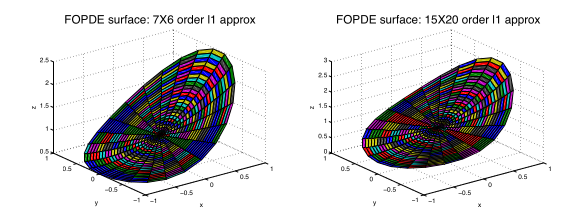
\includegraphics[scale=0.5]{Figures/polejemplo.png}
  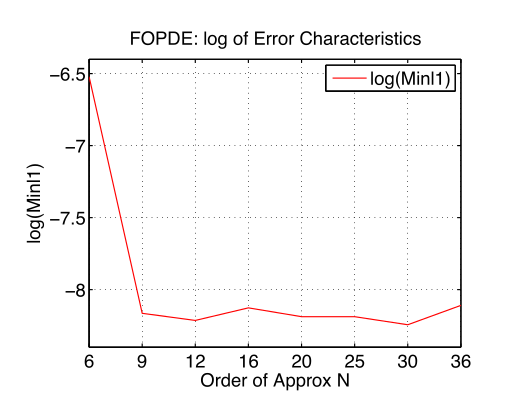
\includegraphics[scale=0.3]{Figures/pol2ejemplo.png}
\end{center}
\end{figure}  
\end{frame}

% Ejemplo y Comparación de Métodos

% Solución de PDEs de segundo orden
\begin{frame}{Resolución de PDEs de Segundo Orden}
    \textbf{Ecuación general:}
    \[
    \Delta u + \alpha (x\partial_x + y\partial_y)^2 u + \beta (x\partial_x + y\partial_y) u + \gamma u = f
    \]
    \textbf{Pasos:}
    \begin{itemize}
        \item Convertir a coordenadas polares y expandir \( u(r, \theta) \) en polinomios de Zernike.
        \item Aplicar integración dos veces para eliminar términos de derivadas de segundo orden.
        \item Transformar la ecuación en un sistema lineal \( Ax = b \) resoluble con métodos numéricos.
    \end{itemize}
\end{frame}

\begin{frame}
  Tras realizar las aproximaciones encontramos cosas como
  \begin{center}
    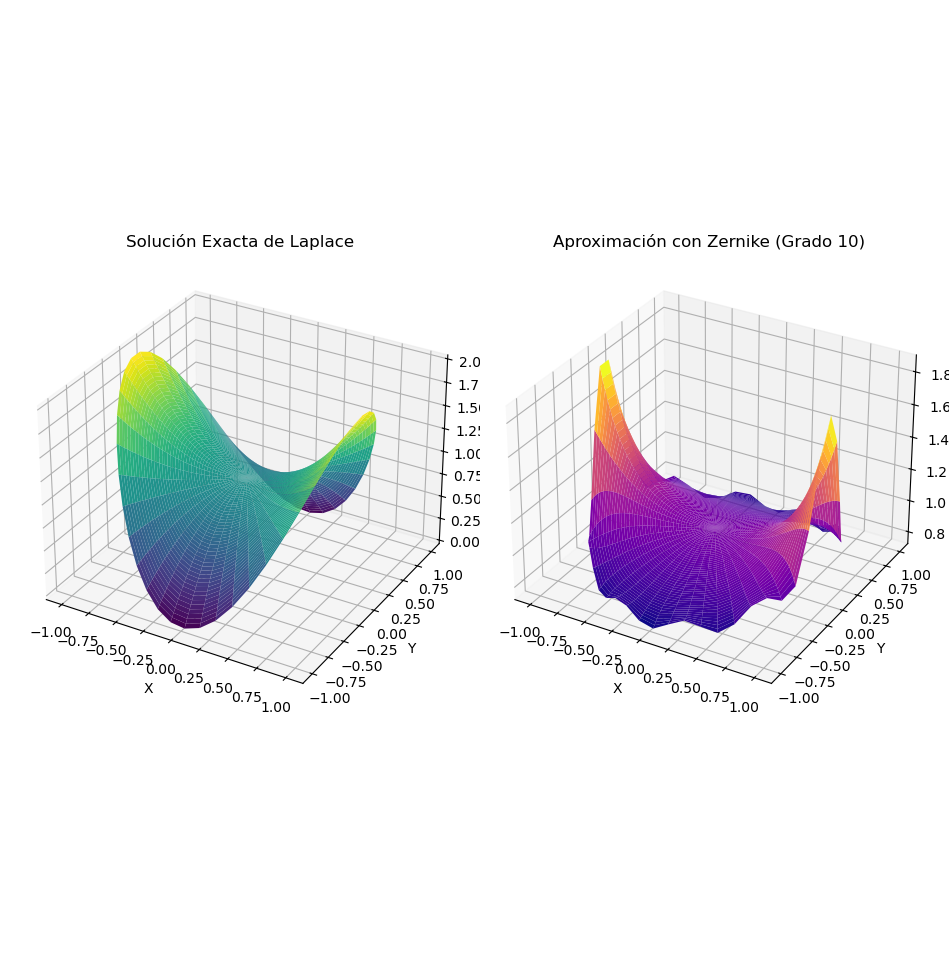
\includegraphics[scale=0.4]{Figures/polortsegundo.png}
  \end{center}
\end{frame}

% Comparación con otros métodos
\begin{frame}{Comparación con Métodos Tradicionales}
    \begin{itemize}
        \item Los métodos espectrales tradicionales (p.ej. Chebyshev) requieren condiciones de frontera bien definidas en puntos específicos.
        \item Las condiciones de frontera discontinuas no pueden manejarse fácilmente con métodos tradicionales.
        \item El uso de polinomios de Zernike permite una mejor representación y aproximación en discos.
    \end{itemize}
\end{frame}

% Conclusiones
\begin{frame}{Conclusiones}
    \begin{itemize}
        \item Se presenta un método eficiente para resolver PDEs en regiones circulares.
        \item Se usa la matriz IOM con polinomios de Zernike para transformar la PDE en un sistema lineal.
        \item Se logra una solución más estable con la minimización \( l_1 \).
        \item Futuras aplicaciones pueden extender este método a ecuaciones más generales en geometrías distintas.
    \end{itemize}
\end{frame}

\begin{frame}[allowframebreaks]
	\frametitle{Bibliografía.}
	
	
	\bibliographystyle{authordate1} 
	%  \bibliographystyle{plain}
	\bibliography{references}
\end{frame}

% Fin de la presentación
\begin{frame}
    \centering
    \Huge ¡Gracias!
\end{frame}

\end{document}

